\documentclass[11pt]{article}
\usepackage[utf8]{inputenc}
\usepackage[T1]{fontenc}
\usepackage{graphicx}
\usepackage[export]{adjustbox}
\graphicspath{ {./images/} }
\usepackage{amsmath}
\usepackage{amsfonts}
\usepackage{amssymb}
\usepackage[version=4]{mhchem}
\usepackage{stmaryrd}

\begin{document}
Overview of Private Equity Funds

This session focuses on the investment pools through which investors gain access to private equity (PE) exposures. The organized PE market is dominated by PE funds. PE funds are unregistered investment vehicles in which investors, or limited partners (LPs), pool money to invest in privately held companies under the management of general partners (GPs). Fund management companies, referred to as PE firms, set up these funds and typically serve as the GPs.

PE funds were discussed at the end of the session, Private Equity Assets as utilizing a potentially superior governance structure for venture capital (VC), growth equity, and buyouts. This session begins with an in-depth discussion of VC funds. Later, leveraged buyout (LBO) funds are detailed.

Start-up ventures have been created and financed throughout history, but the first modern VC firm was American Research and Development, formed in 1946 as a publicly traded closed-end fund. The first VC limited partnership fund was formed in 1958, and the limited partnership form of organization eventually became the standard tool for investing in VC. A VC fund is a PE fund that pools the capital of large sophisticated investors to fund new start-up companies.

\section*{The Organizational Structure of Private Equity Funds}
Each PE fund is managed by a general partner. The general partner is typically the PE firm that raised the capital for the fund. The general partner sources investment opportunities for the fund, reviews business plans, performs due diligence, and, once an investment is made, in the case of a VC fund, typically takes a seat on the board of directors of the start-up company and works with the management of the company to develop and implement the business plan.

PE funds usually have a contractually limited life of seven to 10 years, often with a provision for an extension of two to three years. The VC funds deploy capital by purchasing PE securities in underlying business enterprises, which are referred to as the portfolio companies. VC funds and other PE funds are typically structured as limited partnerships, as discussed in the session, The Environment of Alternative Investments and illustrated in the exhibit, Structure of a Limited Partnership Investment Vehicle for the case of hedge funds. The case of PE is illustrated in the next exhibit.

\begin{center}
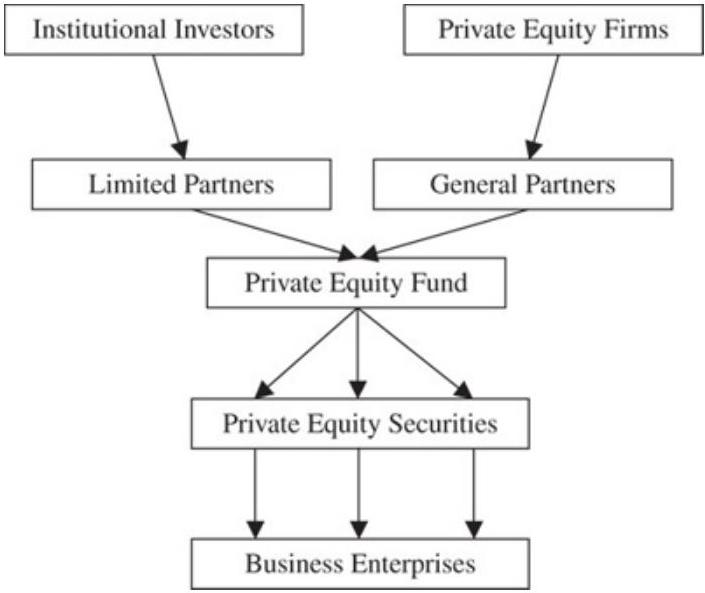
\includegraphics[max width=\textwidth]{2024_04_10_0f4705c4c528462354f4g-2}
\end{center}

\section*{Private Equity Investment Process}
A potentially confusing aspect of PE arises from differentiating between the multiple layers of PE investments. The exhibit above illustrates the three main levels at which PE is discussed. Discussions of PE often refer to the three levels in the above exhibit with interchangeable terms, due in part to the multiple relationships that can exist. Each level is sometimes referred to as PE, and therefore it is sometimes unclear whether the term is being used to describe a manager, an investment fund, or an underlying investment.

At the base of the diagram is the underlying PE investment, which consists of the private business enterprises from which all cash flows to investors must ultimately be derived. Examples include new ventures for VC funds, firms seeking growth equity for growth equity funds, and so forth. The key point is that these are the private enterprises that produce goods or services and that underlie PE investing. The securities of these enterprises (e.g., common stock in these enterprises) are often referred to as PE investments.

The middle level of the above exhibit represents PE funds, which are investment pools created to hold portfolios of PE securities (i.e., the equity securities at the bottom of the exhibit). The funds serve as intermediaries between the underlying business enterprises (called the portfolio companies when they are owned by a fund) and the investors in the PE funds. Institutional investors typically invest in PE as LPs in these funds rather than through direct ownership of PE securities. These PE funds are also often referred to as PE investments.

\section*{Private Equity Firms}
Large PE firms serve as fund managers. The managers serve as GPs and attract institutions as LPs. The fund manager's objective is to realize, or exit, all investments before or at the liquidation of the fund. If successful, the fund managers will launch multiple PE funds through time.

The top right side of the exhibit above depicts PE firms that invest in PE and serve as managers to PE funds. PE firms, such as Kohlberg Kravis Roberts \& Co. (KKR), often serve as the GPs of PE funds, usually invest their own capital, and sometimes fully own the underlying business enterprises. However, PE firms usually obtain additional capital through forming limited partnerships, which attract LPs (e.g., institutions) to invest in a series of ventures. Thus, the Private Equity Investment Process exhibit above depicts both PE firms and institutions investing in PE funds. As indicated in the exhibit, the institutional investors are the LPs.

Typically, a major PE firm serves as the general partner for a series of limited partnerships that span a few decades and may be numbered sequentially or with years (e.g., KKR European Fund III or KKR Fund 1996). Large PE firms may also manage multiple funds concurrently, based on geographic sectors or industry sectors.

Further, the limited partnership funds, indicated as PE funds, in the middle of Private Equity Investment Process are also referred to as PE investments, since the partnership units are usually not publicly traded. Of course, the underlying business enterprises at the bottom of the above exhibit are PE investments. Ownership of these underlying business enterprises is through PE securities, as illustrated with the second to last row of the above exhibit.

The exhibit below provides detail on the entities used to structure the responsibilities and compensation of the relation between the PE firm and the PE fund. The PE firm (which can be an LLC) typically creates an LLC to serve as the general partner (GP) of the partnership. The general partner typically makes a minimal investment in the partnership (e.g., 1\%) but receives a large share (e.g., 20\%) of the distributions (forming the incentive fee). The PE firm typically creates another LLC to serve as the investment adviser to the partnership. The investment adviser receives the management fee (e.g., $2 \%$ annually). As discussed in the session, The Environment of Alternative Investments, the personnel from the PE firm in the LLCs may be overlapping or even identical. The structures are used to preserve limited liability, delineate compensation, and provide clarity with regard to responsibilities.

\begin{center}
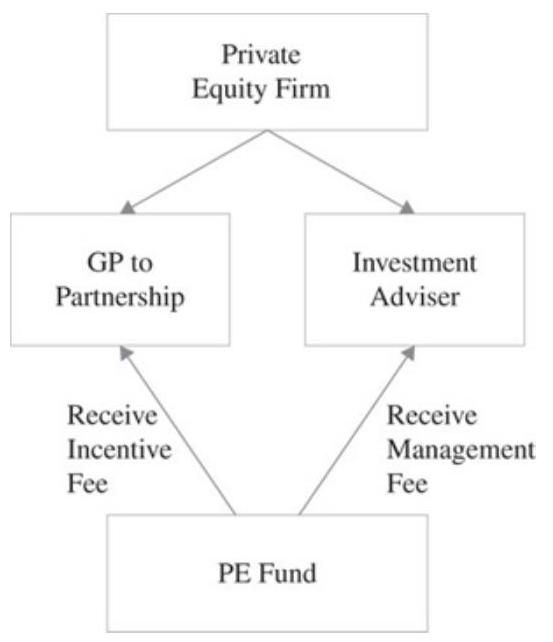
\includegraphics[max width=\textwidth]{2024_04_10_0f4705c4c528462354f4g-3}
\end{center}

\section*{Dual Roles and Entities of a Private Equity Firm}
Tax, legal, and regulatory requirements drive the structuring of the entities in the exhibits, Private Equity Investment Process and Dual Roles and Entities of a Private Equity Firm, as well as goals that include reducing taxation and limiting liability (investors' liabilities are limited to the capital committed to the fund).

The term PE firm is used in this session to describe firms such as KKR at the top level, and the term PE funds is used to describe limited partnerships such as KKR European Fund III at the middle level.

\section*{Private Equity Portfolio Companies}
Finally, PE securities, portfolio companies, or underlying business enterprises are used to describe the underlying investments in the unlisted businesses seeking growth, shown at the bottom level of Private Equity Investment Process exhibit.

In summary, a PE firm creates a PE fund that purchases PE securities. Further, each type of PE investment, such as VC, is sometimes used in place of the more generic term PE. Thus, in the VC area of PE, the concepts illustrated in Private Equity Investment Process exhibit might be referred to as a VC firm creating a VC fund that purchases VC securities.

The structures in the exhibits, Private Equity Investment Process and Dual Roles and Entities of a Private Equity Firm, can be used for growth equity funds and buyout funds as well as VC funds. VC funds can be further distinguished by the stage of VC that the fund focuses on, such as first- or early-stage VC, second- or latestage/expansion VC, and mezzanine financing. Different expertise is required for managing investments at each stage of financing.

A PE limited partnership fund typically invests in 10 to 30 portfolio companies. This translates to approximately two to six companies per year that are sourced, reviewed, and purchased in the first three to five years of the fund's life. In a buyout, the PE fund takes seats on the board of directors. The general partner of the PE firm supplies these new directors, usually picking one to four of its partners to sit on the company's board. As directors, the PE firm interacts with the management of the private company on a weekly, if not daily, basis. A buyout fund assists the company in developing a new business plan. This plan might entail expansion or contraction, adding new employees or deleting part of the workforce, and introducing new products or cutting off unproductive and distracting product development. In a majority of cases, the PE firm gets the company to streamline its workforce, reduce its expenses, and increase its balance sheet capacity for more leverage.

\section*{Private Equity Investment by Institutional Investors}
Many institutions outsource their PE fund investment program either through a dedicated account or by pooling assets with other investors. PE funds of funds are probably the most common type of institutional investment program. PE funds of funds, which are mainly organized by specialist asset managers, are vehicles that pool capital from a group of investors to invest in a diversified portfolio of PE funds. Some funds of funds specialize in certain PE sectors or geographies, whereas others follow a more generalist approach.

PE funds of funds primarily invest in newly formed limited partnerships. Because of the blind pool nature of such investments, in which investors don't know the underlying portfolio companies before committing capital, the initial assessment and ongoing monitoring of the fund management team's skills are key.

PE funds of funds also co-invest alongside primary investors. This activity requires direct investment experience and skills. PE funds of funds can also use secondary investments in existing funds or portfolios of direct investments. This is generally a niche activity for most funds of funds. This activity requires both co-investment skills for the assessment of the companies already in the portfolio and primary investment skills for the blind-pool part of the transaction. Co-investment is discussed in detail in Level II of the CAIA curriculum.

While investment in a particular PE fund can have a blind-pool nature, a fund of funds can have established relationships with fund managers via existing investments. Therefore, its future portfolio is somewhat predictable and is not necessarily a blind pool investment. A newly created portfolio is likely to be largely composed of follow-on funds raised by these known managers. In fact, funds of funds are marketed on either a partially blind or a fully informed basis. For a partially blind pool, some of the intended partnership groups are identified, while for a fully informed pool, virtually all of the intended partnerships have been identified.

Institutions such as pension funds, endowments, PE funds of funds, public institutions, banks, insurance companies, and high-net-worth individuals or family offices invest in PE funds as LPs by committing specified amounts of money to the fund. These commitments are drawn as needed to fund investments. The amount committed but not yet called is an undrawn commitment or dry powder.

For institutional investors, direct investment can be problematic because many institutions cannot offer adequate performance-related pay to attract and retain top employees and analysts. For typical conservative and seniority-based institutions like banks, pension funds, and insurance companies, a theoretically unlimited carried interest does not always fit well with the institution's traditional compensation scheme.

While institutional investors do not lack staff with the intellectual caliber to evaluate investment proposals and to structure transactions, generating profitable exits in PE programs requires very hard work over protracted periods of time. Moreover, the lack of incentive to take risk and to find value (or the conflict of interest therein) may affect investment decisions.

There is a substantial learning curve, and without performance-related pay, employees may jump ship as soon as they are competent in the area and understand their opportunities better. Finally, for larger institutions, intermediation through funds of funds allows them to focus on their core businesses.


\end{document}